\chapter{Обзор состояния проблемы и постановка задачи исследования}

Современный уровень науки и технологий характеризуется
широким использованием нелинейных динамических
систем~\cite{andronov_vitt_haikin,anisch_nonlin_eff,mishenko_du_small_relax,nonlin_vibro,malinetskii_modern_methods_nl_dyn}.
При этом нелинейные эффекта присущи как объектам,
так и системам управления~\cite{kubik_nlsc,vukobr_nonadopt}. Динамика нелинейных систем,
характеризуется общим уровнем сложности моделей,
в большинстве случаев не допускающего
точного аналитического представления.
Помимо этого, был обнаружен, и в последнее время представляет
постоянный интерес для исследователей класс систем,
проявляющих хаотическую динамику~\cite{moon_chaotic_vibr,magni_theory_dyn_chaos,kuznetsov_dyn_chaos,neimark_stoch_chaos_vibro,anisch_reg_and_chaotic_vibro}.
Для таких систем, вследствие чувствительности к начальным условиям
и параметрам, характерным свойством является наличие ограниченного горизонта прогноза как
в прошлое, так и в будущее, рост энтропии
и необратимость процессов~\cite{chernavskii_syn_info,prigogine_from_existent,koltsova_nl_dyn_chem}.
Это свойство делает неприменимыми
большинство методов, разработанных для описания, управления и
идентификации динамических систем. Также было замечено,
что некоторые известные динамические системы, в том числе широко
используемые в научной, производственной и технологической практике,
зарекомендовавшие себя как системы регулярной динамики,
при определённых условиях демонстрируют хаотическое поведение.
Хаотически свойства проявляют системы как классической,
так и квантовой механики.
Новые свойства подобных систем требуют создания новых
методов для решения задач моделирования,
управления и идентификации~\cite{karabutov_adapt_id_sys,dmitriev_trans_chaos_lowpower}.


\section{Основные понятия задачи идентификации динамических систем} % {{{1

Одно из первых определений задачи идентификации было дано
Л.~Заде~\cite{zadeh_id_1956}.
Согласно этому определению,
``Идентификация состоит в отыскании по входным и выходным сигналам
некоторой системы эквивалентной ей системы
из некоторого заданного класса''~\cite{eykhoff_id_base,eykhoff_modern_id,lung_id_sys}.


Н.С.~Райбман в предисловии к известной работе П.~Эйкхоффа~\cite{eykhoff_id_base}
дал следующее определении идентификации
``по результатам наблюдений над входными и выходными переменными системы должна быть
построена оптимальная в некотором смысле модель, то есть формализированное представление этой системы''.
Данное определение отличается предельной широтой охвата за счёт того,
что под определение ``оптимальная в некотором смысле'' попадает
практически любое, в том числе не относящееся к собственно идентификации условие.
В одной из последующих работ~\cite{raibman_id_obj_ctl}
вид этого определения стал более строгим и формальным:
``В качестве критерия оптимальности используется функция выходных переменных объекта $y(t)$ и модели
$y^{*}(t) = A_t^{*} x(s) $, и на ёё математическое ожидание накладывается условие
$M \{\rho [ y_t, y_t^{*} ] \} \to {\min}$''.
Это определение действительно соответствует задаче идентификации ценой
введения существенных ограничений: возможности представления динамики системы в виде оператора,
существования и возможности определения математического ожидания,
и соответствия минимума этого ожидания близости динамики системы и её модели.



Определение Растригина.



Критерии

% TODO: may be p1?
При описании и анализе динамики хаотических
систем используются специализированные характеристики и показатели.
Например, сечение Пуанкаре~\cite{moon_chaotic_vibr,anisch_complex_vibrations_in_simple_systems,atu_st105}
позволяет визуально определить признаки хаотической динамики.
Однако, использование визуальных признаков в качестве критерия
весьма затруднено.

Другим важным признаком является фрактальная размерность. %TODO: cite
В отличие от сечения Пуанкаре, она имеет скалярный вид,
что делает возможным её использование в качестве критерия.
Однако, диапазон изменения этой величины для большинства сигналов достаточно мал,
и в условиях шумов измерения выделить полезную
для идентификации составляющую весьма затруднительно.

% }}}1

\section{Существующие методы идентификации нелинейных динамических систем и их свойства}  % {{{1

Ввиду того, что задача идентификации сложных динамических систем всегда была актуальной,
и привлекала внимание многих исследователей, было создано
значительное количество методов и систем идентификации.
Создание универсальной системы идентификации, безусловно подходящей для
любой динамической системы, представляется практически нерешаемой задачей.
Следовательно, каждый из существующих методов имеет свою область применения.
Наиболее математически обоснованным являются методы идентификации
линейных систем.
Для очень узкого класса нелинейных систем является возможным
получение аналитического выражения для значения параметра
по измерениям входных и выходных сигналов. Чаще всего,
для сложных динамических систем получить такую аналитическую
зависимость невозможно. Поэтому широкое распространение получили методы
с использованием параллельной модели, % TODO: cite
в которых на вход и модели, и объекта подаётся один и тот же входной сигнал,
и параметры модели настраиваются таким образом, чтобы выход модели
был наиболее близким к выходу объекта. В какой-то мере
именно такие методы отображают определение идентификации.
Между собой эти методы отличаются способами настройки параметров модели.


\subsection{Синхронный детектор} % {{{2

Принцип работы синхронного детектора %  \cite{adopt_cont_sys}
(рис.~\ref{atu:f:syncdet})
заключается в том,
что значение коэффициента модели модулируется либо гармоническим,
либо случайным сигналом. Для выявления влияния
изменения коэффициента на ошибку идентификации
производится перемножение модулирующего сигнала с ошибкой
идентификации. После усреднения данного сигнала
получаем оценку значения градиента функции ошибки на
пространстве параметров.

\begin{figure}[htb!]
\begin{center}
% vi:syntax=tex
\begin{tikzpicture}
  % \draw[hair,step=1.0em] (0,-3) grid (12.0,3.0);
  \bXStyleBloc{semiboldline,inner sep=2pt};
  \bXLineStyle{medline};
  % --- U
  \bXInput{U};
  \path (U.center) ++(2.5em,0.0em) coordinate (UxM);
  \draw (U.center) -- (UxM);
  \fill (UxM) circle[radius=0.05];
  \node[above right] at(U) {$u(t)$};
  % --- Obj
  \bXBranchy[-3]{UxM}{U0};
  % \fill[red](U0) circle[radius=0.05];
  \bXBlocL[1.0]{Obj}{$\mathbf{O}$}{U0};
  \bXLinkyx{UxM}{Obj};
  % --- M1
  \bXBranchy[3]{UxM}{U1};
  %\fill[green](U1) circle[radius=0.05];
  \bXBlocL[1.0]{M1}{$\mathbf{M}$}{U1};
  \bXLinkyx{UxM}{M1};
  % --- W
  \bXCompSum[5.0]{W}{Obj}{}{}{}{};
  \bXLink[$x_o(t)$]{Obj}{W};
  \path (W.north) ++(0.0em,2.0em) coordinate (Win);
  \draw[medlinep] (Win) -- (W.north);
  \node[below right] at(Win) {$w(t)$};
  % --- Err
  \bXCompSum[9.5]{Err}{UxM}{+}{-}{}{};
  \bXLinkxy{W}{Err};
  \bXLinkxy{M1}{Err};
  \node[above right] at(M1.east) {$x_m(t)$};
  % --- Mult
  \bXCompSum*[9.0]{Mult}{Err}{}{}{}{};
  \bXLink[$e(t)$]{Err}{Mult};
  %\fill[black](Mult) circle[radius=0.07];
  \node at(Mult) {$\times$};
  % --- LPF
  \bXBloc[2.0]{LPF}{\textbf{LPF}}{Mult};
  \bXLink{Mult}{LPF};
  % --- Mixer
  \bXBranchy[6]{Mult}{MixPoint};
  \bXCompSum[0.0]{Mixer}{MixPoint}{}{}{}{};
  % \bXReturn{LPF}{Mixer}{};
  \bXLinkyx{LPF}{Mixer};
  % --- param
  \draw[semiboldlinep] (Mixer.west) -| (M1.south);
  \node[below right] at(M1.south east) {$p(t)$};
  % --- Gener
  \bXBranchy[3]{Err}{GenPoint};
  \bXBloc[2]{Gener}{\textbf{G}}{GenPoint};
  \bXLinkxy[$g(t)$]{Gener}{Mult};
  \bXLinkxy{Gener}{Mixer};
  \fill (Mixer) ++(0.0em,3.0em) circle[radius=0.05];
  %
  \TikzAddPadding
  %
\end{tikzpicture}

\end{center}
\caption{Система идентификации с синхронным детектором}
\label{atu:f:syncdet}
\end{figure}

%В
%\cite{Eykhoff,adopt_cont_sys}
показано, что в квазистационарных условиях
происходит смещение рабочей точки системы идентификации
в направлении градиента функции качества,
со скоростью, пропорциональной значению модуля этого градиента.

% }}}2

\subsection{Метод идентификации с переменной частотой пробного воздействия} % {{{2

Принцип работы данного метода
% (рис.~\ref{f:vsf1})
основан на том, что на параметрический вход модели подаётся треугольный поисковый сигнал.
Этот сигнал генерируется специальным генератором,
состоящего из управляемого генератора прямоугольных колебаний, 
счётного триггера и интегратора%  \cite{auto_optim_intask,adopt_cont_sys}.

% \begin{figure}[htb]
% \centerline{
%  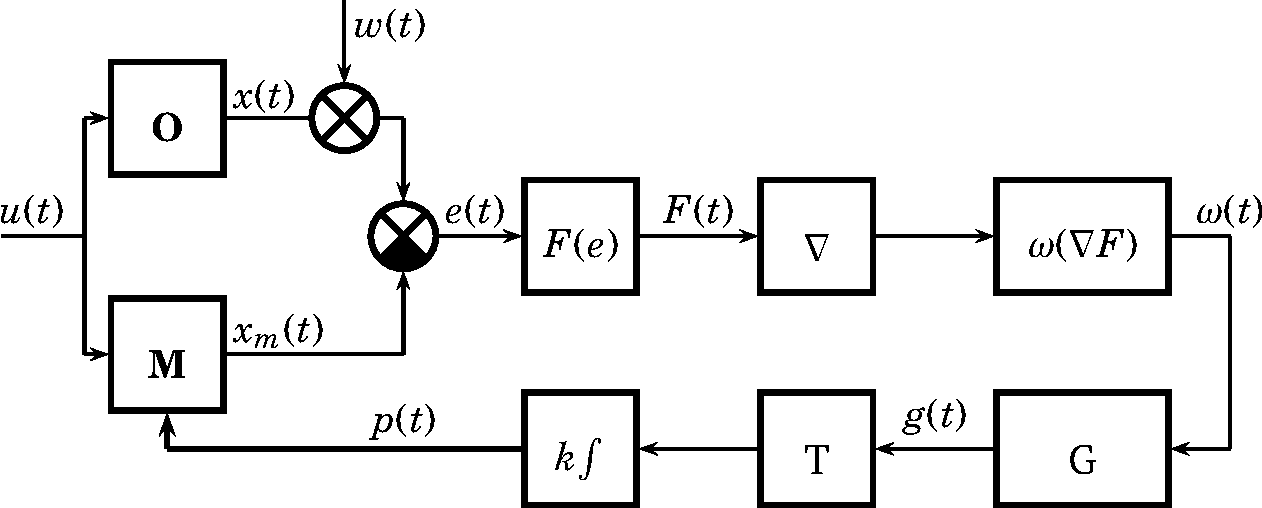
\includegraphics[width=11cm]{lpics/vsf1.eps}
%  %\resizebox{11.0\scm}{!}{%
%  %  \input{lpics/vsf1.tex}
%  %}
% }
% \caption{Система идентификации с переменной частотой пробного воздействия}
% \label{f:vsf1}
% \end{figure} 

Результаты предварительного моделирования показали,
что данный метод, хоть и показывает хорошие результаты
в задачах оптимизации, но для решения задач идентификации 
практически не применим. Наличие дифференцирующего 
звена делает данный метод особо чувствительным к шумам
измерения, а в задачах идентификации с параллельной моделью
влияние входного сигнала \( u(t) \)
на ошибку измерения \( e(t) \) 
имеет вид мультипликативного шума,
что полностью нарушает процесс поиска.

% }}}2

\subsection{Метод случайного поиска} % {{{2

Основа данного метода заключается в том, что
очередном шаге сравнивается текущее и предыдущее
значения ошибки идентификации, и решение о смешении
рабочей точки принимается в соответствии с выбранной
тактикой случайного поиска.
% \cite{rastr_rand_search_adopt,rastr_intro,ivanov_stoh_alg_int}.

Наиболее известными и распространённым
являются линейная и нелинейная тактика
%\cite{rastr_rand_search,gladkov_optim_nongrad}.
При использовании линейной тактики
в случае уменьшения ошибки идентификации
производится шаг в том же направлении, что и предыдущий.
В противном случае производится случайный шаг.
При использовании нелинейной тактики
случайный шаг делается в случае уменьшения ошибки.
В противном случае делается шаг назад.

Метод имеет широкий диапазон применимости,
но проявляет свои преимущества на сложных 
системах с большим количеством идентифицируемых параметров.
В более простых случаях проявляется такой недостаток,
как малая скорость поиска.

% }}}2

\subsection{Непараметрические методы} % {{{2

При использовании этого метода идентификации
роль модели играет нейронная сеть
% (рис.~\ref{f:neuro})
% \cite{bodyan_osn_theor_ann,nelles_nlsys_id,chen_nls_id_radial_basis}.
Коэффициенты нейронной сети настраиваются каким-либо
известным алгоритмом таким образом, чтобы
достичь минимума ошибки.

Использование нейронной сети в качестве модели позволяет иметь дело с
объектами, структура которых неизвестна или же слишком сложна для построения
традиционной модели.

При этом результат подобной идентификации сложно, а зачастую и невозможно
применить где-либо, кроме имитационного моделирования.  Структура и
коэффициенты нейронной сети не дают представления о структуре объекта и его
параметрах.  При проведении идентификации с использованием нейросетевой модели
в достаточно сложных случаях нет гарантии завершения процесса настройки сети и
затруднительно оценить скорость поиска при настройке сети.

С точки зрения информационных критериев оценки качества систем идентификации,
нейросетевая идентификация в большинстве случает не даёт непосредственной
информации об параметрах изучаемого объекта.  В данной работе такие методы
рассматриваться не будут.

Тем не менее, нейронные сети можно использовать для настройка коэффициентов
традиционной модели.  Такое использование может быть оправдано, если ввиду
большой размерности выходного сигнала \(x\) или других причин, нет возможности
сформировать скалярный критерий качества. В таком случае на первый слой
нейронной сети можно подавать по-координатно выходы модели и объекта и
проводить настройку нейронной сети таким образом, чтобы её выходные сигналы (а
следовательно, и коэффициенты модели) обеспечивали минимум какого-либо
синтетического критерия.

% }}}2

\subsection{Адаптивно-поисковая идентификация с возмущением параметра одной модели} % {{{2

Метод адаптивно-поисковой идентификации с возмущением параметров одной модели
изначально был разработан как метод поисковой оптимизации
% \cite{mai_adopt_meth_direct,ivah_int_meth_direct,mai_iss_adop_alg_etalon,rastr_seu}.
\cite{mich_92}
Минимальные требования к априорной информации, хорошая помехоустойчивость и
простота схемотехнической реализации позволили применить данный метод не только
для решения задач оптимизации, но и для задач идентификации параметров сложных
систем
%\cite{mai_akt_meth_sear,mai_sear_meth_akt,mai_akt_id_robot,ivah_alg_id_parm,mai_sear_meth_akt_id_ns}.


% }}}2

\subsection{Адаптивно-поисковая идентификация с возмущением параметра пары моделей} % {{{2
 Self
% }}}2

Основы идентификации систем управления~\cite{eykhoff_id_base,eykhoff_modern_id,gropp_methods_id,deith_method_id_ds,lung_id_sys,seidg_id_su,leondes_modern_tu,nelles_nlsys_id}

Введение в идентификацию объектов управления~\cite{rastr_intro,rastr_adop_complex_sys}.

Случайный поиск в задачах оптимизации многопараметрических систем~\cite{rastr_rand_search,rastr_rand_search_adopt}.

Статистические методы поиска~\cite{rastr_stat_meth_search}

Беспоисковые самонастраивающиеся системы~\cite{kozlov_nosearch_sns}

Системы экстремального управления~\cite{rastr_seu,kras_dyn_nsn}

Основы информационной теории идентификации~\cite{info_cipkin,straton_inf,karabut}

Адаптация в непрерывных системах автоматического поиска~\cite{adopt_cont_sys}

Карабутов~\cite{karabutov_adapt_id_sys,saliga_id_ctl_black}

Козлов~\cite{kozlov_nosearch_sns} -- беспоисковые.

Растригин~\cite{rastr_stat_meth_search,rastr_seu,rastr_intro,rastr_adop_complex_sys,rastr_rand_search}

Борцов~\cite{borcov} -- эле-мех.

Автоматическая оптимизация в задачах пространственного распределения~\cite{auto_optim_intask}


% }}}1

\section{Свойства систем хаотической динамики применительно к задаче идентификации}  % {{{1

Одним из основных свойств систем хаотической динамики является чувствительность
к малым возмущениям сходных сигналов, состояния системы или же параметров.
В линейном приближении это соответствует положительным значениям
коэффициентов Ляпунова~\cite{magni_theory_dyn_chaos,moon_chaotic_vibr}.


% }}}1

\section{Постановка задачи исследования}  % {{{1

Критерии.

Методы.

Средства моделирования и измерения.

Проверка адекватности.


% }}}1

\section{Постановка задачи идентификации}  % {{{1

Пусть задан динамический объект $ \mathbf{O}$, характеризуемый параметром $p_o(t)$.
Информация об этом параметре может быть представлена
различными способами. Например, может быть задан только диапазон
$[p_{\min}, p_{\max}]$,
возможных значений параметра,
этот же диапазон может иметь зависимость от времени:
$[p_{\min}(t), p_{\max}(t)]$.
Множество допустимых значений параметра обозначим через $\mathcal{P}$.
На основании априорных исследований может
быть задана как плотность вероятности для значений параметра,
так и зависимость этой вероятности от времени. Наличие плотности вероятности
позволяет использовать информационные оценки идентификации~\cite{info_cipkin,atu_asau10},
но не является необходимым условием для синтеза системы идентификации в целом.
Более того, для получения достаточно точных информационных оценок
требуется затратить значительно больше ресурсов на проведение моделирования,
чем на собственно идентификацию.
Также могут быть заданы дополнительные ограничения, такие как максимальна скорость
изменения параметра и т.д.

Пусть также существует конечное множество моделей
\label{atu:d:N}$\mathbf{M}_i$, $i=0 \ldots N-1$.
Структура моделей предполагается известной и одинаковой,
а параметру объекта $p_o(t)$ соответствуют параметры моделей $p_{i}(t)$.

На вход как моделей, так и объекта подаётся входной сигнал \label{atu:d:u}$u(t)$.
Частный случай, когда ни объект, ни модели не требуют входного сигнала
не нарушает общности постановки. В некоторых случаях
не следует пренебрегать ошибкой измерения входного сигнала $w_u(t)$,
однако, при анализе динамики систем идентификации в целом,
этой величиной, как правило, пренебрегают.

В общем случае $u(t)$, $x(t)$, $p(t)$ -- векторные величины.
В тех случаях, когда размерность $x(t)$ не выше трёх,
компоненты этого вектора будем обозначать соответственно $x(t)$, $y(t)$, $z(t)$.

Выходные сигналы моделей
\label{atu:d:x}$x_i(t)$ считаем известными точно, так как ошибки
представления значений при численных вычислениях заведомо
пренебрежимо малы с точностью измерений. Напротив,
выход объекта $x_{op}(t)$ считаем измеренным
с определённой ошибкой измерения \label{atu:d:w}$w(t)$:
%
\[
  x_o(t) = x_{op}(t) + w(t).
\]
%
Сигнал $w(t)$ обычно задаётся как случайный сигнал с
известным видом распределения, а также параметрами этого распределения,
например, нормальное распределения с среднеквадратичным отклонением $\sigma_w$
и характерным временем автокорреляции $\tau_w$.
При моделировании процессов измерения внешних сигналов в помощью АЦП может потребоваться
более сложное представление:
%
\[
  x_o(t) = W( x_{op}(t) + w(t) ).
\]
%
Данный способ определения $x_o(t)$ необходим в тех случаях,
когда надо отобразить при моделировании тот факт,
что данный сигнал принимает фиксированный набор значений, определяемый разрядностью АЦП.

Временные ограничения на работу системы идентификации могут быть заданы
следующими способами. В простейшем случае, значение $p_o$
считается постоянным, но ограничено полное время измерения $T$.
В противном случае задаются ограничения на динамику $p_o(t)$.
Распространённые способы:

a) ограничение производной:
%
\begin{equation}
  \left| \od{p_o(t)}{t} \right| < d_{p,\max}.
  \label{atu:eq:p_lim_diff}
\end{equation}
Самый простой метод, но имеет ограниченное применение в реальных
задачах, так как резкие изменение значений параметра,
связанные с переключениями состояния или режимов работы системы,
выходом из строя элементов системы на дают возможности корректно ограничить
величину  $d_{p,\max}$. С другой стороны, такие изменения
происходят достаточно редко, и этот факт не отражает ограничение (\ref{atu:eq:p_lim_diff}).

b) ограничение длины кривой $p_o(t)$ на любом из интервалов времени $[t,t+\Delta t]$:
\begin{equation}
  \int\limits_{t}^{t+\Delta t} \sqrt{1 + \left( \od{p_o(t)}{t} \right)^2 } \, \mathrm{d}t < l_{p,\max}.
  \label{atu:eq:p_lim_l}
\end{equation}
%
Это ограничение выглядит несколько искусственным,
но оно, с одной стороны, вводит ограничение на возможные изменения $p_o(t)$,
и с другой стороны, не ограничивает резкие изменения параметра в отдельных областях.

c) упрощённая форма варианта b) -- ограничение длины проекции  $p_o(t)$ на ось $p$:
\begin{equation}
  \int\limits_{t}^{t+\Delta t} \left| \od{p_o(t)}{t} \right | \, \mathrm{d}t < l_{pl,\max}.
  \label{atu:eq:p_lim_pl}
\end{equation}

Целью задачи идентификации будем считать нахождение
такого сигнала $p_\mathrm{id}(t)$, для которого
отличие $q_\mathrm{id}(t)$ от $q_o(t)$ минимально.
Понятие ``отличие'', как и вид критерия $q$, определяется исходной задачей.







% }}}1


\section{Выводы по разделу \thechapter}  % {{{1


% }}}1


% vim: fdm=marker foldlevel=0 foldignore="%#" fdc=4 ft=tex
